\documentclass[a4paper,UTF8]{article}
\usepackage{ctex}
\usepackage[margin=1.25in]{geometry}
\usepackage{color}
\usepackage{graphicx}
\usepackage{amssymb}
\usepackage{amsmath}
\usepackage{amsthm}
\usepackage{enumerate}
\usepackage{bm}
\usepackage{hyperref}
\usepackage{epsfig}
\usepackage{color}
\usepackage{mdframed}
\usepackage{lipsum}
\usepackage{mathtools}
\usepackage{hyperref}
\usepackage{diagbox}
\usepackage{float}
\usepackage{caption}
\usepackage{algorithm}
\usepackage{algorithmicx}  
\usepackage{algpseudocode}
\usepackage{amsmath} 
\usepackage{graphicx}
\usepackage{subfigure}
\newmdtheoremenv{thm-box}{myThm}
\newmdtheoremenv{prop-box}{Proposition}
\newmdtheoremenv{def-box}{定义}
\usepackage{listings}
\usepackage{xcolor}
\lstset{
	numbers=left, 
	numberstyle= \tiny, 
	keywordstyle= \color{ blue!70},
	commentstyle= \color{red!50!green!50!blue!50}, 
	frame=shadowbox, % 阴影效果
	rulesepcolor= \color{ red!20!green!20!blue!20} ,
	escapeinside=``, % 英文分号中可写入中文
	xleftmargin=2em,xrightmargin=2em, aboveskip=1em,
	framexleftmargin=2em
} 

\usepackage{booktabs}

\setlength{\evensidemargin}{.25in}
\setlength{\textwidth}{6in}
\setlength{\topmargin}{-0.5in}
\setlength{\topmargin}{-0.5in}

% \setlength{\textheight}{9.5in}
%%%%%%%%%%%%%%%%%%此处用于设置页眉页脚%%%%%%%%%%%%%%%%%%
\usepackage{fancyhdr}                                
\usepackage{lastpage}                                           
\usepackage{layout}                                             
\footskip = 10pt 
\pagestyle{fancy}                    % 设置页眉                 
\lhead{研一下学期}                    
\chead{论文阅读笔记}                                                
% \rhead{第\thepage/\pageref{LastPage}页} 
\rhead{Step5}                                                                                               
\cfoot{\thepage}                                                
\renewcommand{\headrulewidth}{1pt}  			%页眉线宽,设为0可以去页眉线
\setlength{\skip\footins}{0.5cm}    			%脚注与正文的距离           
\renewcommand{\footrulewidth}{0pt}  			%页脚线宽,设为0可以去页脚线

\makeatletter 									%设置双线页眉                                        
\def\headrule{{\if@fancyplain\let\headrulewidth\plainheadrulewidth\fi%
\hrule\@height 1.0pt \@width\headwidth\vskip1pt	%上面线为1pt粗  
\hrule\@height 0.5pt\@width\headwidth  			%下面0.5pt粗            
\vskip-2\headrulewidth\vskip-1pt}      			%两条线的距离1pt        
 \vspace{6mm}}     								%双线与下面正文之间的垂直间距              
\makeatother  

%%%%%%%%%%%%%%%%%%%%%%%%%%%%%%%%%%%%%%%%%%%%%%
\numberwithin{equation}{section}
%\usepackage[thmmarks, amsmath, thref]{ntheorem}
\newtheorem{theorem}{Theorem}
\newtheorem*{definition}{Definition}
\newtheorem*{solution}{Solution}
\newtheorem*{prove}{Proof}
\newcommand{\indep}{\rotatebox[origin=c]{90}{$\models$}}

\usepackage{multirow}

%--

%--
\begin{document}
\title{论文阅读笔记\\
Step5}
\author{MF1833063, 史鹏, spwannasing@gmail.com}
\maketitle

\newpage
\section{ERNIE:Enhanced Language Representation with Informative Entities}
此文章是对bert的一次扩展,提出了知识图谱中的多信息实体(informative entity)可以作为外部知识改善语言表征。
\begin{figure}[H]
	\centering
	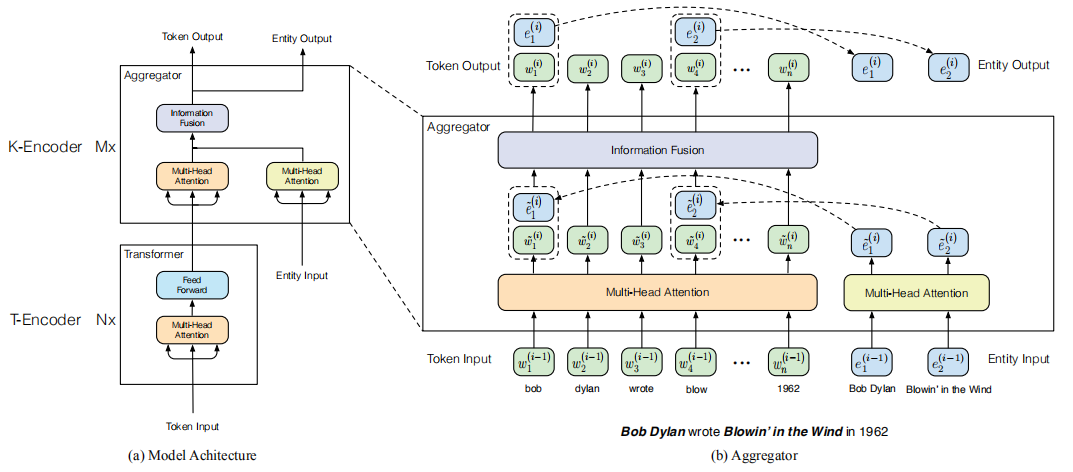
\includegraphics[width=\textwidth]{1-1.png}
	\caption{overview}
\end{figure}
\begin{figure}[H]
	\centering
	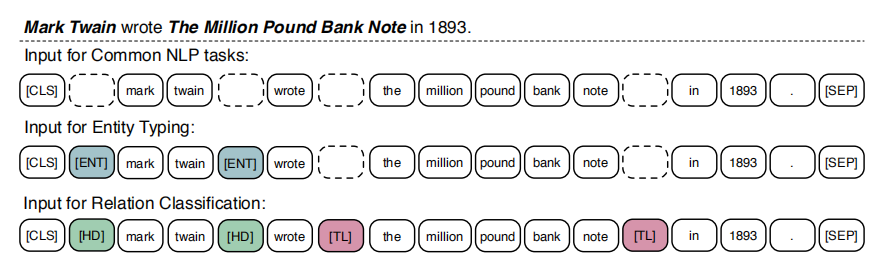
\includegraphics[width=\textwidth]{1-2.png}
	\caption{finetune}
\end{figure}
Knowledgeable Encoder:
\begin{equation}
	\left\{\tilde{\boldsymbol{w}}_{1}^{(i)}, \ldots, \tilde{\boldsymbol{w}}_{n}^{(i)}\right\}=\mathrm{MH}-\mathrm{A} \mathrm{T} \mathrm{T}\left(\left\{\boldsymbol{w}_{1}^{(i-1)}, \ldots, \boldsymbol{w}_{n}^{(i-1)}\right\}\right)
	\end{equation}
	\begin{equation}
		\left\{\tilde{e}_{1}^{(i)}, \ldots, \tilde{e}_{m}^{(i)}\right\}=\operatorname{MH}-\operatorname{ATT}\left(\left\{e_{1}^{(i-1)}, \ldots, e_{m}^{(i-1)}\right\}\right)
		\end{equation}

对于和entity对齐的token:
\begin{equation}
\begin{aligned} \boldsymbol{h}_{j} &=\sigma\left(\tilde{\boldsymbol{W}}_{t}^{(i)} \tilde{\boldsymbol{w}}_{j}^{(i)}+\tilde{\boldsymbol{W}}_{e}^{(i)} \tilde{\boldsymbol{e}}_{k}^{(i)}+\tilde{\boldsymbol{b}}^{(i)}\right) \\ \boldsymbol{w}_{j}^{(i)} &=\sigma\left(\boldsymbol{W}_{t}^{(i)} \boldsymbol{h}_{j}+\boldsymbol{b}_{t}^{(i)}\right) \\ \boldsymbol{e}_{k}^{(i)} &=\sigma\left(\boldsymbol{W}_{e}^{(i)} \boldsymbol{h}_{j}+\boldsymbol{b}_{e}^{(i)}\right) \end{aligned}
\end{equation}

else:
\begin{equation}
\begin{aligned} \boldsymbol{h}_{j} &=\sigma\left(\tilde{\boldsymbol{W}}_{t}^{(i)} \tilde{\boldsymbol{w}}_{j}^{(i)}+\tilde{\boldsymbol{b}}^{(i)}\right) \\ \boldsymbol{w}_{j}^{(i)} &=\sigma\left(\boldsymbol{W}_{t}^{(i)} \boldsymbol{h}_{j}+\boldsymbol{b}_{t}^{(i)}\right) \end{aligned}
\end{equation}

对于引入的信息的pre-training目标:
\begin{equation}
	p\left(e_{j} | w_{i}\right)=\frac{\exp \left(\text { linear }\left(\boldsymbol{w}_{i}^{o}\right) \cdot \boldsymbol{e}_{j}\right)}{\sum_{k=1}^{m} \exp \left(\text { linear }\left(\boldsymbol{w}_{i}^{o}\right) \cdot \boldsymbol{e}_{k}\right)}
	\end{equation}

\newpage
\section{ERNIE: Enhanced Representation through Knowledge Integration}
ERNIE 通过建模海量数据中的词、实体及实体关系,学习真实世界的语义知识。相较于 BERT 学习原始语言信号,ERNIE 直接对先验语义知识单元进行建模,增强了模型语义表示能力。
这里我们举个例子:\\

Learnt by BERT :哈 [mask] 滨是 [mask] 龙江的省会,[mask] 际冰 [mask] 文化名城。\\

Learnt by ERNIE:[mask] [mask] [mask] 是黑龙江的省会,国际 [mask] [mask] 文化名城。\\

在 BERT 模型中,我们通过『哈』与『滨』的局部共现,即可判断出『尔』字,模型没有学习与『哈尔滨』相关的任何知识。而 ERNIE 通过学习词与实体的表达,使模型能够建模出『哈尔滨』与『黑龙江』的关系,学到『哈尔滨』是 『黑龙江』的省会以及『哈尔滨』是个冰雪城市。

训练数据方面,除百科类、资讯类中文语料外,ERNIE 还引入了论坛对话类数据,利用 DLM(Dialogue Language Model)建模 Query-Response 对话结构,将对话 Pair 对作为输入,引入 Dialogue Embedding 标识对话的角色,利用 Dialogue Response Loss 学习对话的隐式关系,进一步提升模型的语义表示能力。

我们在自然语言推断,语义相似度,命名实体识别,情感分析,问答匹配 5 个公开的中文数据集合上进行了效果验证,ERNIE 模型相较 BERT 取得了更好的效果。
\begin{figure}[H]
	\centering
	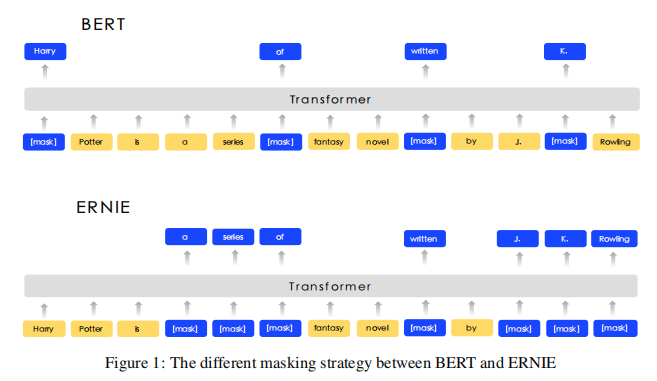
\includegraphics[width=\textwidth]{2-1.png}
\end{figure}
\begin{figure}[H]
	\centering
	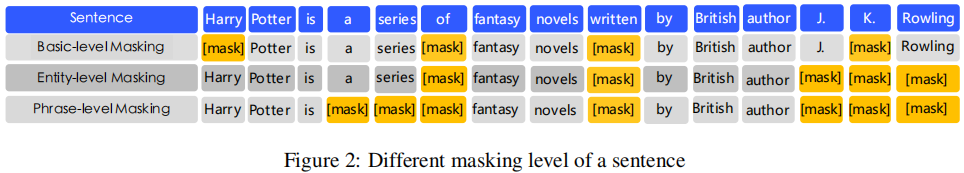
\includegraphics[width=\textwidth]{2-2.png}
\end{figure}
\begin{figure}[H]
	\centering
	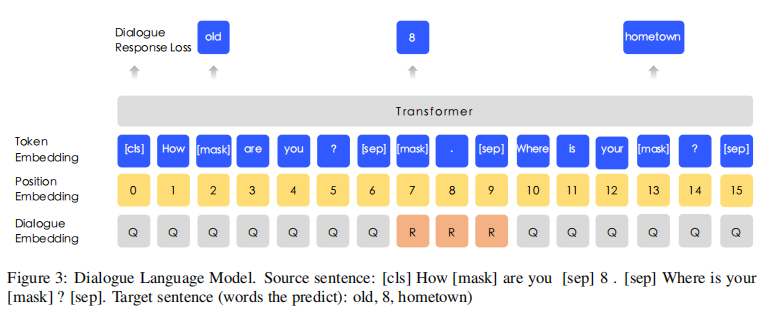
\includegraphics[width=\textwidth]{2-3.png}
\end{figure}


\newpage
\section{Learning to Ask Unanswerable Questions for Machine Reading Comprehension}
提出一种数据增强技术,根据与包含答案的相应段落配对的可回答问题自动生成相关的无法回答的问题。所提出的结构为“pair-to-sequence”。
\begin{figure}[H]
	\centering
	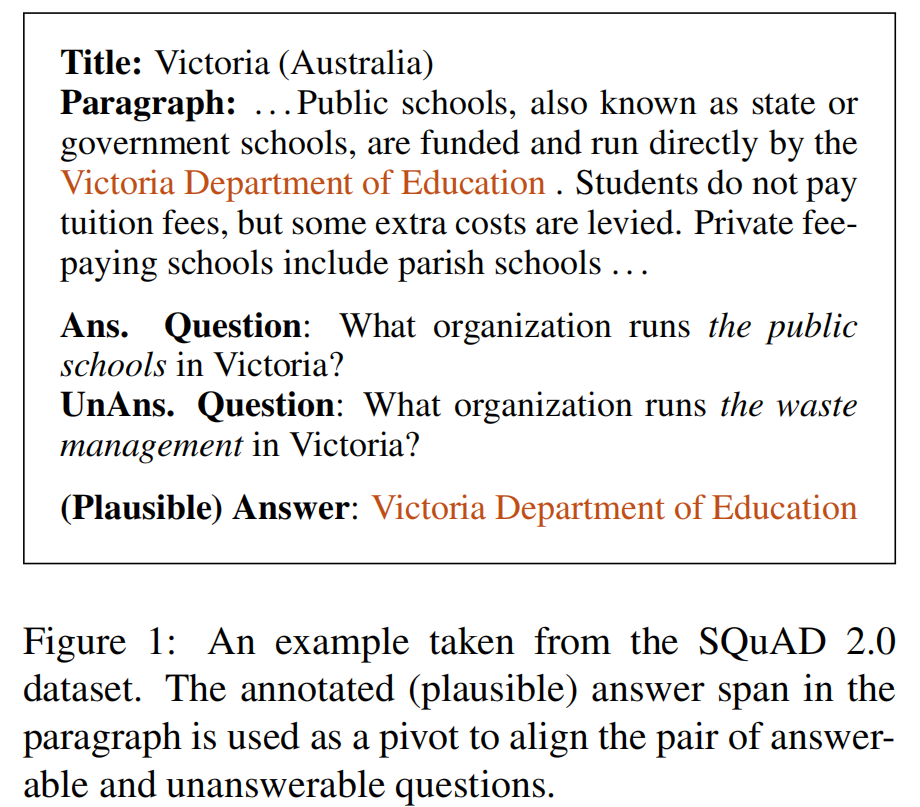
\includegraphics[width=0.6\textwidth]{3-1.png}
\end{figure}
\begin{figure}[H]
	\centering
	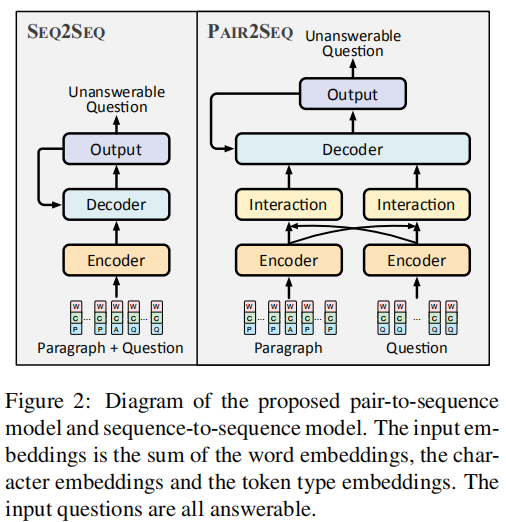
\includegraphics[width=0.6\textwidth]{3-2.png}
\end{figure}

\newpage
\section{Course Concept Expansion in MOOCs with External Knowledge and Interactive Game}
随着大规模在线开放课程(MOOC)的日益普及,为MOOC用户自动提供课外知识成为可能。语义漂移和知识缺乏在复杂的MOOC环境下,现有的方法不能有效地扩展课程概念。
本文首先在通过外部知识库搜索新概念的过程中建立一个新的边界,然后利用异构特征来验证高质量的结果。具体算法没有特别仔细地看。
\begin{figure}[H]
	\centering
	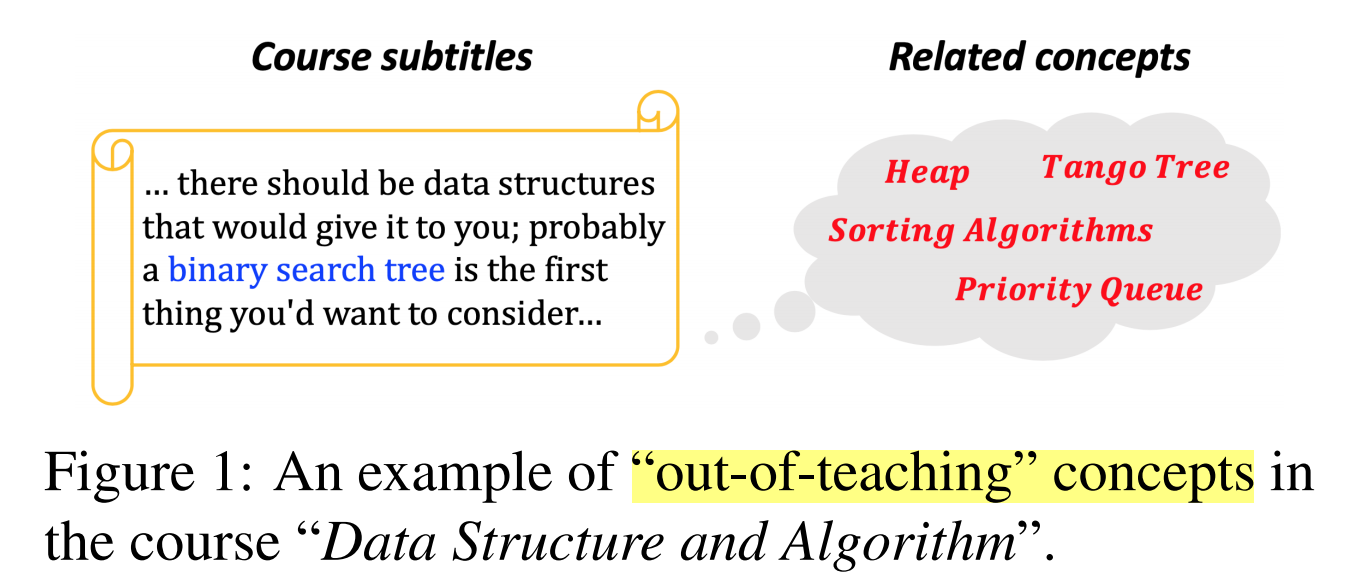
\includegraphics[width=0.6\textwidth]{4-1.png}
\end{figure}

\newpage
\section{XLNet: Generalized Autoregressive Pretraining for Language Understanding}
本文提出了一个新的预训练模型,在20个任务上刷新了Bert的记录。其相对bert的主要改进是结合了AR(Transformer-XL)和AE的优点,抛弃了bert的Masked language model,使用了Permutation language model。
对于每一种排列的序列,并不是改变原始的序列(即position embedding不变),只是改变mask(bert里的mask是直接mask一个word,这里的是在Transformer的计算过程中“mask”住不需要的部分)。
e.g 在图二中,对于序列3241,1能“看见”324,所以都不用mask掉,而对于2,只能看见3,所以要mask掉14。

虽然排列语言模型能满足目前的目标,但是对于普通的transformer结构来说是存在一定的问题的,为什么这么说呢,看个例子,假设我们要求这样的一个对数似然,$p_{\theta}\left(X_{z_{t}} | x_{z_{<t}}\right)$如果采用标准的softmax的话,那么

$$
p_{\theta}\left(X_{z_{t}} | x_{z_{<t}}\right)=\frac{\exp \left(e(x)^{T} h_{\theta}\left(x_{z_{z}}\right)\right)}{\sum_{x^{\prime}} \exp \left(e\left(x^{\prime}\right)^{T} h_{\theta}\left(x_{z_{<t}}\right)\right)}
$$

其中$h_{\theta}\left(x_{z_{<t}}\right)$表示的是添加了mask后的transformer的输出值,可以发现$h_{\theta}\left(x_{z_{<t}}\right)$并不依赖于其要预测的内容的位置信息,因为无论预测目标的位置在哪里,因式分解后得到的所有情况都是一样的,并且transformer的权重对于不同的情况是一样的,因此无论目标位置怎么变都能得到相同的分布结果,如下图所示,假如我们的序列index表示为[1,2,3],对于目标2与3来说,其因式分解后的结果是一样的,那么经过transformer之后得到的结果肯定也是一样的。
\begin{figure}[H]
	\centering
	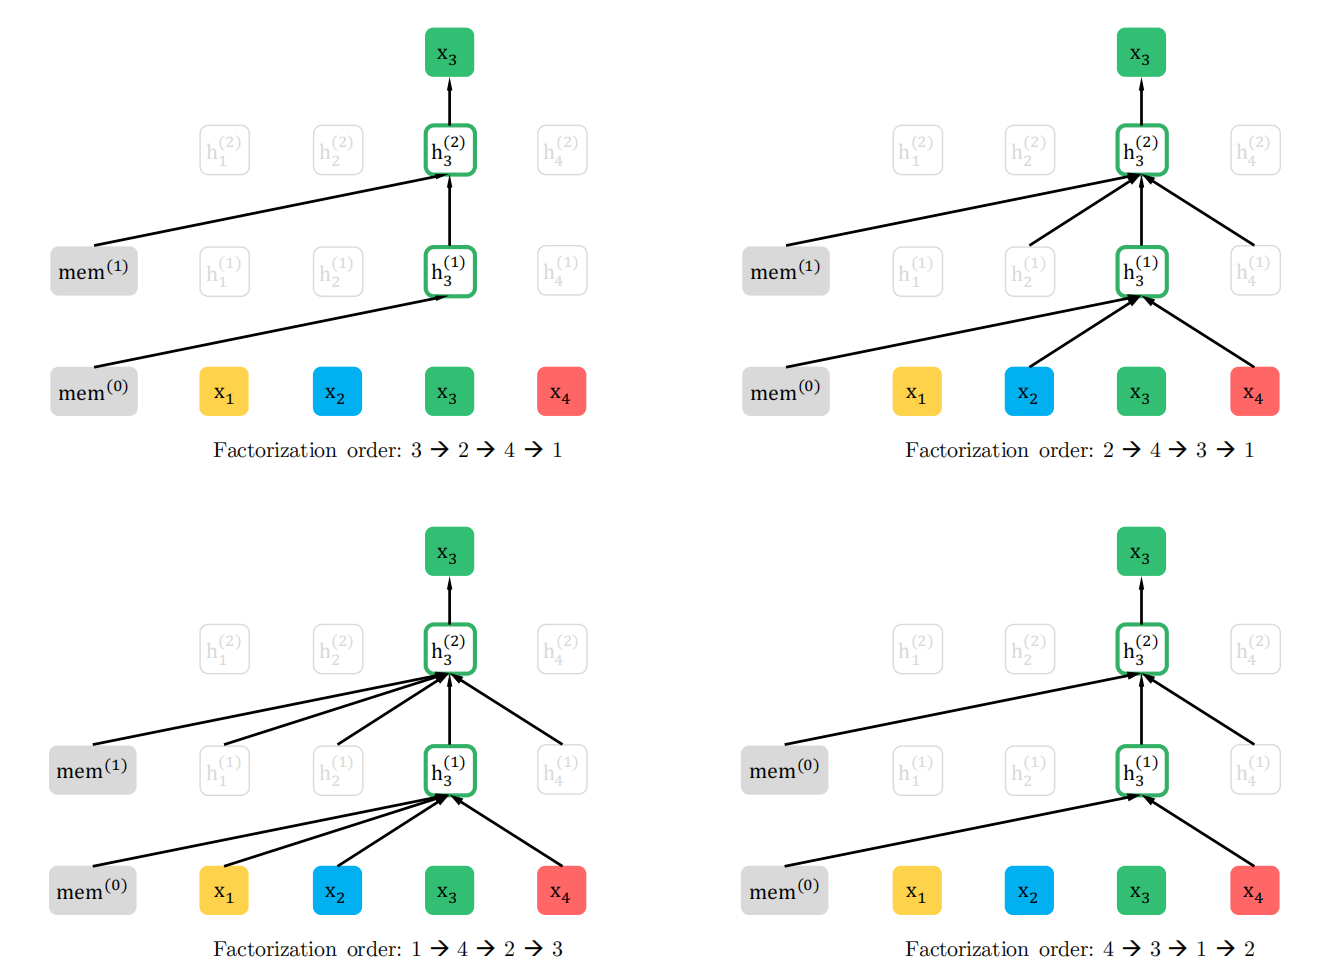
\includegraphics[width=\textwidth]{5-1.png}
\end{figure}

因此就提出了基于目标感知表征的双流自注意力。
$$
\begin{array}{l}{g_{z_{t}}^{(m)} \leftarrow \text { Attention }\left(\mathrm{Q}=g_{z_{t}}^{(m-1)}, \mathrm{KV}=\mathbf{h}_{\mathrm{z}<t}^{(m-1)} ; \theta\right)} \\ {h_{z_{t}}^{(m)} \leftarrow \text { Attention }\left(\mathrm{Q}=h_{z_{t}}^{(m-1)}, \mathrm{KV}=\mathrm{h}_{\mathrm{z} \leq t}^{(m-1)} ; \theta\right)}\end{array}
$$
\begin{figure}[H]
	\centering
	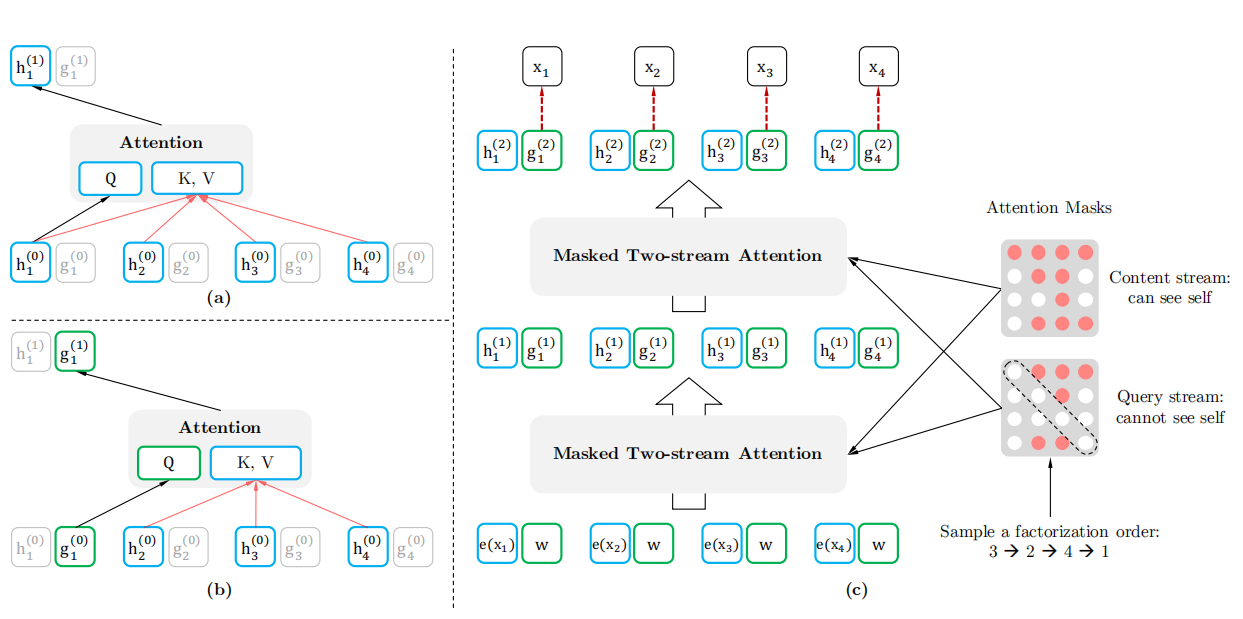
\includegraphics[width=\textwidth]{5-2.png}
\end{figure}

reference:\\
https://zhuanlan.zhihu.com/p/70257427 \\
https://blog.csdn.net/u012526436/article/details/93196139


\newpage
\section{Star-Transformer}
本文提出了一种对于Transformer改进的结构“star-Transformer”。将标准Transformer中全连接的部分调整为星型的拓扑结构,在实际任务中速度提升了4.5倍。
\begin{figure}[H]
	\centering
	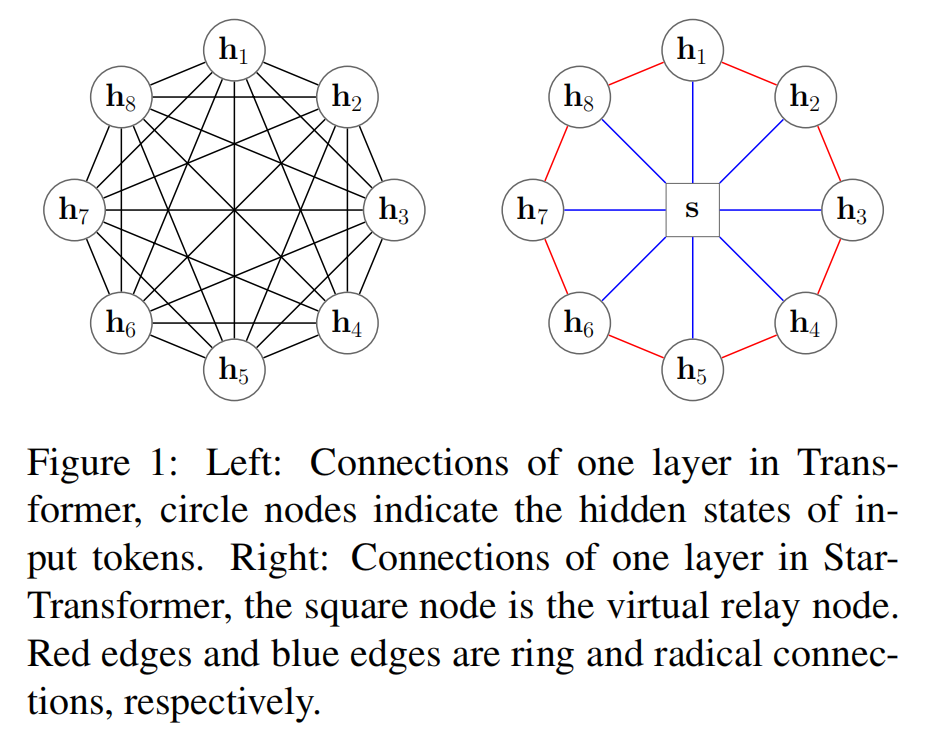
\includegraphics[width=0.6\textwidth]{6-1.png}
\end{figure}

添加了一个虚拟的节点作为relay node。由此可以分为两种连接,Radical Connections和Ring Connections。环连接可以有效地减少局部和非局部成分的非偏置学习负担,提高模型的泛化能力。
将标准的Transformer复杂度 $O(n^2)$降低为$O(n)$。

根式连接集中在非局部构图上,环连接集中在局部构图上。因此,star-Transformer适用于尺寸适中的数据集,不依赖于繁重的预培训。

令$\mathbf{s}^{t} \in \mathbb{R}^{1 \times d}$ and $\mathbf{H}^{t} \in \mathbb{R}^{n \times d}$ 分别为relay node和所有的satellite node。

初始化$\mathbf{H}^{0}=\mathbf{E}$ 和 $s^0 = \text{average}(\mathbf{E})$

$$
\begin{array}{l}{\mathbf{C}_{i}^{t}=\left[\mathbf{h}_{i-1}^{t-1} ; \mathbf{h}_{i}^{t-1} ; \mathbf{h}_{i+1}^{t-1} ; \mathbf{e}^{i} ; \mathbf{s}^{t-1}\right]} \\ {\mathbf{h}_{i}^{t}=\text { MultiAtt }\left(\mathbf{h}_{i}^{t-1}, \mathbf{C}_{i}^{t}\right)}\end{array}
$$
$$
\mathbf{h}_{i}^{t}=\text { LayerNorm }\left(\operatorname{ReLU}\left(\mathbf{h}_{i}^{t}\right)\right), i \in[1, n]
$$
$$
\begin{array}{l}{\mathbf{s}^{t}=\text { MultiAt }\left(\mathbf{s}^{t-1},\left[\mathbf{s}^{t-1} ; \mathbf{H}^{t}\right]\right)} \\ {\mathbf{s}^{t}=\text { LayerNorm (ReL } \mathrm{U}\left(\mathbf{s}^{t}\right) )}\end{array}
$$
\end{document}